\section{Durchführung}
\label{sec:Durchführung}


\begin{figure}
    \centering
    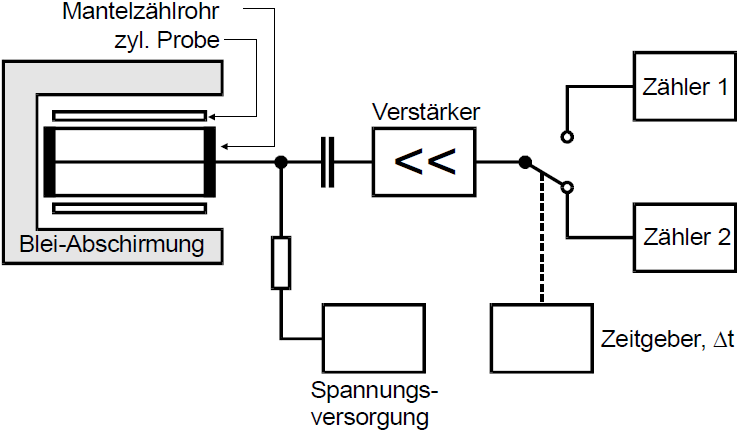
\includegraphics[width=\textwidth]{data/aufbau.png}
    \caption{Schematischer Aufbau des Versuchs \cite{V702}}
    \label{fig:aufbau}
\end{figure}

Die Erzeugung von Neutronen erfolgt, indem $\ce{^{9}_{4}Be}$-Kerne mit $\alpha$-Teilchen beschossen werden, 
wobei die Reaktion 
\begin{equation}
    \ce{^{9}_{4}Be} + \ce{^{4}_{2}\alpha} \longrightarrow \ce{^{12}_{6}Be} + \ce{^{1}_{0}n}
\end{equation}
erfolgt. Die $\alpha$-Teilchen kommen durch den Zerfall von $\ce{^{226}Ra} $ zustande. Die Geschwindigkeit dieser wird dann gesenkt, indem ein Paraffinmantel die Neutronenquelle umgibt. Paraffin wird 
gewählt, da es zum großen Teil aus Wasserstoff besteht, was der ideale Stoßpartner für die Neutronen ist. Beim durchdringen 
dieser Schicht geben die Neutronen durch Stoßprozesse einen Teil ihrer Energie ab, wodurch sie an Geschwindigkeit verlieren bis 
diese etwa $\SI{2.2}{\kilo\metre\per\s} $ bei $T=\SI{290}{\kelvin} $ beträgt. Ein solches Neutron wird dann als thermisches 
Neutron bezeichnet. Die Abbildung \ref{fig:aktivierung} zeigt den schematischen Aufbau eines dafür zuständigen Aktivierungsbehälters
im Querschnitt. 
\begin{figure}
    \centering
    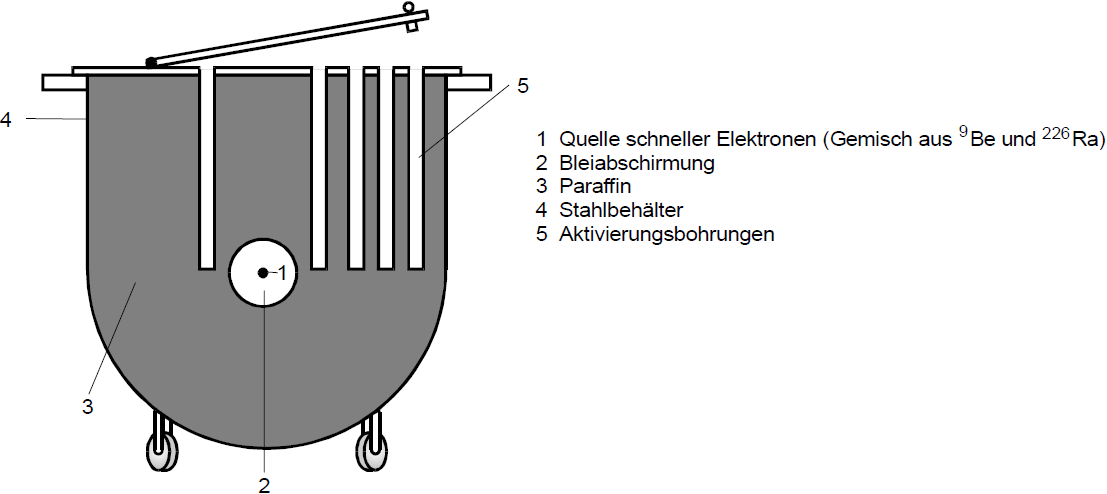
\includegraphics[width=\textwidth]{data/aktivierung.png}
    \caption{Skizze des Aktivierungsbehälters im Querschnitt \cite{V702}}
    \label{fig:aktivierung}
\end{figure}
\FloatBarrier
Der Zerfall der Atomkerne, der durch den Beschuss mit Neutronen zustande kommt, siehe Gleichung \ref{sec:Theorie}, wird durch ein 
Geiger-Müller-Zählrohr registriert. Dieser leitet das Signal an zwei alternierende Zähler weiter. Zwischen diesen wird im Zeitintervall
$\Delta t$ umgeschaltet, um eine ununterbrochene Messung zu gewährleisten und die Notierung der Messwerte zu erleichtern.
So kann die Größe $N_{\Delta t}(t) $ bei festgelegtem Zeitintervall gemessen werden. Das Geiger-Müller-Zählrohr befindet sich dabei 
samt Probe in einem Bleimantel, um äußere Strahlungseinwirkung zu minimieren. Um diese Strahlungseinwirkung trotzdem mit 
einbeziehen zu können, wird der Nulleffekt $N_U$ gemessen, indem das Geiger-Müller-Zählrohr insgesamt sieben mal über ein 
Zeitintervall von $\Delta t =\SI{300}{\s} $ eine Messung ohne Preparat die auftreffenden Impulse misst. Dies muss in der Auswertung der Messergebnisse 
berücksichtigt werden.
\\
Um die Halbwertszeit von Vanadium zu untersuchen, wird die Vanadiumprobe in den Aufbau integriert. Dies erfolgt möglichst schnell,
nachdem die das Preparat durch den Neutronenbeschuss aktiviert wurde. Die Messzeit für das zählen der Zerfälle beträgt hierbei 
$\Delta t= \SI{30}{\s} $ und es werden die Zerfälle für 42 Intervalle gemessen. Für die Untersuchung von Rhodium ist die 
Vorgehensweise identisch, nur dass diesmal das Zeitintervall der Messung $\Delta t= \SI{30}{\s} $ beträgt. Auch diese Messung 
erstreckt sich über 42 Intervalle.